% This is text associated with the open textbook "Open Electromagnetics"
% See immediately below for author, date
% This work is licensed under the Creative Commons Attribution-ShareAlike 4.0 International License. (CC BY SA 4.0) 
% To view a copy of the license, visit http://creativecommons.org/licenses/by-sa/4.0/

%ORB TITLE Inductance of a Straight Coil
%ORB AUTHOR 0        # S.W. Ellingson, Virginia Tech (ellingson@vt.edu)
%ORB DATE 20180804   # yyyymmdd
%ORB ABSTRACT Inductance of a Straight Coil

\label{m0124_Inductance_of_a_Straight_Coil} % <-- Must match name of this file and module directory name.  Don't mess with this!
\index{inductor!straight coil|(}

In this section, we determine the inductance of a straight coil, 
\index{coil}
as shown in Figure~\ref{m0124_fCoil}.
The coil is circular with radius $a$ and length $l$ and consists of $N$ windings of wire wound with uniform winding density.
Also, we assume the winding density $N/l$ is large enough that magnetic field lines cannot enter or exit between windings but rather must traverse the entire length of the coil.
Since the coil forms a cylinder, the problem is easiest to work in cylindrical coordinates with the axis of the coil aligned along the $z$ axis.
%
\begin{figure}[b!]
\begin{center}
\pdftooltip{{  % note double braces
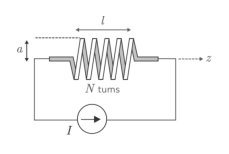
\includegraphics[width=2.5in]{modules/m0124_fCoil.eps}
}}{A circular coil with radius a and length l, consisting of N turns wound uniformly lies on the z-axis in a series circuit with current pointed to the right running counterclockwise.}
\end{center} 
% ***WikipediaCommonsURL
%\centerline{\scriptsize 
%\copyright~\hyperref[m0124_fCoil_Credit]{author} 
%\href{https://creativecommons.org/licenses/by-sa/4.0/}{CC BY~SA 4.0} 
%}
\caption{
\label{m0124_fCoil}
Determination of the inductance of a straight coil.
}
\end{figure}  

Inductance $L$ in this case is given by (Section~\ref{m0123_Inductance})
%
\begin{equation}
L = \frac{N\Phi}{I}
\label{m0124_eLdef}
\end{equation} 
%
where $I$ is current and $\Phi$ is the magnetic flux associated with one winding of the coil.  Magnetic flux in this case is given by
%
\begin{equation}
\Phi = \int_{\mathcal S}{\bf B}\cdot d{\bf s}
\end{equation}
%
where ${\bf B}$ is the magnetic flux density (units of T = Wb/m$^2$), ${\mathcal S}$ is the surface bounded by a single current loop, and $d{\bf s}$ points in the direction determined by the right hand rule with respect to the direction of positive current flow.

First, let's determine the magnetic field.
The magnetic flux density deep inside the coil is (Section~\ref{m0120_Magnetic_Field_of_a_Coil}):
%
\begin{equation}
{\bf B} \approx \hat{\bf z}\frac{\mu NI}{l} 
\label{m0124_eBapprox}
\end{equation}
%
Is it reasonable to use this approximation here?  
Since inductance pertains to energy storage, the question is really what fraction of the energy is stored in a field that is well-described by this approximation, as opposed to energy stored in the ``fringing field'' 
\index{fringing (field)}
close to the ends of the coil.  If we make $l$ sufficiently large relative to $a$, then presumably energy storage in the fringing field will be negligible in comparison.  Since the alternative leads to a much more complicated problem, we shall assume that Equation~\ref{m0124_eBapprox} is valid for the interior of the coil.

Next, we determine $\Phi$.
In this case, a natural choice for ${\mathcal S}$ is the interior cross-section of the coil in a plane perpendicular to the axis.
The direction of $d{\bf s}$ must be $+\hat{\bf z}$ since this is the direction in which the fingers of the right hand point when the current flows in the direction indicated in Figure~\ref{m0124_fCoil}.
Thus, we have
%
\begin{flalign}
\Phi &\approx \int_{\mathcal S}\left(\hat{\bf z}\frac{\mu NI}{l}\right)\cdot \left(\hat{\bf z}ds\right) \nonumber \\
~~ &= \frac{\mu NI}{l} \int_{\mathcal S}ds \nonumber \\
~~ &= \frac{\mu NI}{l}A 
\end{flalign} 
%
where $A$ is the cross-sectional area of the coil. 

Finally from Equation~\ref{m0124_eLdef} we obtain
%
\begin{equation}
\boxed{
L \approx \frac{\mu N^2 A}{l} ~~(l\gg a)
}
\label{m0124_eLlsc}
\end{equation} 
%
Note that this is dimensionally correct; that is, permeability (units of H/m) times area (units of m$^2$) divided by length (units of m) gives units of H, as expected.
Also, it is worth noting that inductance is proportional to permeability and cross-sectional area, and inversely proportional to length.
Interestingly the inductance is proportional to $N^2$ as opposed to $N$; this is because field strength increases with $N$, and independently there are $N$ flux linkages.
Finally, we note that the inductance does not depend on the \emph{shape} of the coil cross-section, but only on the \emph{area} of the cross-section.
Summarizing:
%
%ORB HIGHLIGHT
\begin{mdframed}[backgroundcolor=yellow!20,nobreak=true] 
The inductance of a long straight coil is given approximately by Equation~\ref{m0124_eLlsc}. 
\end{mdframed}

Again, this result is approximate because it neglects the non-uniform fringing field near the ends of the coil and the possibility that magnetic field lines escape between windings due to inadequate winding density.
Nevertheless, this result facilitates useful engineering analysis and design.

%------------------------------------

{\bf Additional Reading:}
\begin{itemize}
\item ``\href{https://en.wikipedia.org/wiki/Inductance}{Inductance}'' on Wikipedia.
\end{itemize}

\index{inductor!straight coil|)}
